\documentclass{beamer}
\usetheme{Madrid}
\usecolortheme{default}
\usepackage{graphicx} % Required for inserting images
\graphicspath{ {./images/} }
\usepackage{geometry}
\usepackage[T1]{fontenc}
\usepackage{fbb}
\usepackage{amsthm}
\usepackage[libertine]{newtxmath} 
\usepackage[italic]{mathastext}
\MTsetmathskips{f}{5mu}{1mu} 
\usepackage[utf8]{inputenc}
\usepackage{textcomp}
\usepackage{graphicx}
\usepackage{amssymb} 
\def\acts{\curvearrowright}
\usepackage{listings}
\usepackage{caption}
\usepackage{subcaption}
\usepackage{lipsum}
\usepackage{setspace}
\usepackage{chngcntr}
\usepackage{faktor}
\usepackage{fancyhdr}
\usepackage{listings}
\usepackage{multirow}
\usepackage{scalerel}
\DeclareMathOperator*{\bigplus}{\scalerel*{+}{\sum}}
\usepackage{tikz-cd}
\usetikzlibrary{patterns.meta}
\usepackage{hyperref}


\title{
    The Hypercubic Manifold\\
    in\\
    Homotopy Type Theory}
\date{04/09/2023}
\author{{Dylan Laird} \\ 
{\and} \\
{Supervisors} \\
{Samuel MIMRAM} \\ {Emile OLEON}}
\institute{LIX, Polytechnique}

\begin{document}

\frame{\titlepage}

\begin{frame}
    \frametitle{Table of contents}
    \tableofcontents
\end{frame}
\AtBeginSection[]
{
  \begin{frame}
    \frametitle{Table of contents}
    \tableofcontents[currentsection]
  \end{frame}
}
\section{Intro}
\begin{frame}
    \frametitle{Intro (1) : HoTT }
    \begin{exampleblock}{Homotopy Type Theory}
        \begin{itemize}
            \item Vladimir Voevodsky : proposed the "Univalence Axiom"
            \pause
            \item Synthetic homotopy
            \pause
            \item Computer assisted proofs
            \pause
            \item "Univalent Foundations" as a foundational system for maths
        \end{itemize}
    \end{exampleblock}
\end{frame}
\begin{frame}
    \frametitle{Intro (2) : Homotopy theory}
    Let $X$ be a topological space and $I$ the unit real interval $[0,1]$
    \pause
    \begin{itemize}
        \item Paths:  continuous maps $p : I \rightarrow X$
        \pause
        \item Homotopy : describes the correct notion of "equality" for paths. \\
        \pause
        \item Two paths $p$ and $q$ are "homotopic" if there is "a continuous deformation" of $p$ onto $q$
        \pause
        \item Loops: a loop at point $x$ is a path $p$ such that $p(0)=p(1)=x$.
    \end{itemize}
\end{frame}
\begin{frame}
    \frametitle{Intro (3) : Homotopy theory}
    \begin{figure}[h]
        \centering
        \begin{tikzpicture}[scale=1.5]
          \draw (0,0) ellipse (3.5cm and 2cm);
          \filldraw (-2.5,0) circle (1.5pt) node [below left] {$x$};
          \filldraw (2.5,0) circle (1.5pt) node [below right] {$y$};
          \filldraw [pattern={Lines[angle=60, distance=8pt]}] (-2.5,0) .. controls (-1,1.5) and (1,1.5) .. (2.5,0) .. controls (1,-1.5) and (-1,-1.5) .. (-2.5,0) -- cycle;
          \draw [thick, double] (0,1.152) -- (0,-1.152) node [at start, above] {$p$} node [midway, right] {$H$} node [at end, below] {$q$};
          \node (A) at (3.3,1.5) {$X$};
        \end{tikzpicture}
    \end{figure}
\end{frame}
\begin{frame}
    \frametitle{Intro (4) : Homotopy theory}
    \begin{exampleblock}{Paths operations}
        \begin{itemize}
            \item inversion : given $p : x \rightarrow y$ there is a path $p^{-1} : y \rightarrow x$
            \item concatenation : given $p : x \rightarrow y$ and $ q : y \rightarrow z$ there is a path $ p \cdot q : x \rightarrow z$
        \end{itemize}
    \end{exampleblock}
    \pause
    \begin{alertblock}{Fundamental group $\pi_1(X,x)$
        }
        Take a point $x$ of $X$ and consider loops at point $x$.
        \begin{itemize}
            \item Equality: homotopy (of loops)
            \item Composition : path concatenation (associative)
            \item Inverse element : inverse path
            \item Unit element : constant path at $x$
        \end{itemize}
        Two (path connected) homeormorphical spaces (more precisely, homotopically equivalent) have the same fundametal groups !
    \end{alertblock}
\end{frame}
\begin{frame}
    \frametitle{Intro (5) : Homotopy theory}
    \begin{exampleblock}{Higher homotopy groups}
        \begin{itemize}
            \item Homotopy are themselves paths between paths
            \pause
            \item We can then take a look at fundamental groups based at a certain loop $\gamma$ and elements of this group will be homotopies between $\gamma$ and itself and so on...
            \pause
            \item  We can define higher homotopy groups $\pi_n(X,x)$ for any $n \in \mathbb{N}^*$ with $n=1$ being the fundamental group.
        \end{itemize}
    \end{exampleblock}
    \pause
    \begin{exampleblock}{Natural questions}
        \begin{itemize}
            \item Given a finite group $G$ is there a (path-connected) space $X$ such that $\pi_1(X) = G$ ?
            \pause
            Answer : yes (cell-complexes)
            \pause
            \item Is there a (path-connected) space such that $\pi_1(X)=G$ and $\pi_n(X)=1$ for any $n\geq 2$ ?
            \pause Answer : yes, the \textbf{Eilenberg Mac-Lane} space of $G$ 
        \end{itemize}
    \end{exampleblock}
\end{frame}
\begin{frame}
    \frametitle{Intro (6) : What's the connection with type theory ?}
    We manipulate types $A,B$ and terms $a : A$ of some certain type. \\
    \pause
    \begin{exampleblock}{The inductive type of natural integers}
        \begin{itemize}
            \item $0 : \mathbb N$
            \item $\mathrm{suc}: \mathbb N \rightarrow \mathbb N$
        \end{itemize}
    \end{exampleblock}
    \pause
    \begin{block}{Equality}
        We distinguish between \textbf{definitional equality} $\equiv$ used when defining objects and \textbf{propositional equality} which is a type theoretical concept.
    \end{block}
    \pause
    \begin{exampleblock}{Propositional Equality}
        Given a type $A$ and terms $a,b : A$ there is a type $a=_A b$. We say that elements $a$ and $b$ are (propositionally) equal when there exists some element  : $$p : a=_A b$$
    \end{exampleblock}
\end{frame}
\begin{frame}
    \frametitle{Intro (7) : What's the connection with Type Theory ?}
    \begin{center}
        \begin{tabular}{|c|c|}
        \hline Types & Topology  \\
        \hline$A$ & a space $A$   \\
        \hline$a: A$ & $a$ is a point of $A$ \\
        \hline $p : x=_A y$ & $p$ is a path from $x$ to $y$ in the space $A$ \\
        \hline
        \end{tabular}
    \end{center}
    \pause
    \begin{figure}[h]
        \centering
        \begin{tikzpicture}[scale=0.7]
          \draw (0,0) ellipse (3.5cm and 2cm);
          \filldraw (-2.5,0) circle (1.5pt) node [below left] {$x$};
          \filldraw (2.5,0) circle (1.5pt) node [below right] {$y$};
          \filldraw [pattern={Lines[angle=60, distance=8pt]}] (-2.5,0) .. controls (-1,1.5) and (1,1.5) .. (2.5,0) .. controls (1,-1.5) and (-1,-1.5) .. (-2.5,0) -- cycle;
          \draw [thick, double] (0,1.152) -- (0,-1.152) node [at start, above] {$p$} node [midway, right] {$r$} node [at end, below] {$q$};
          \node (A) at (3.3,1.5) {$A$};
        \end{tikzpicture}
    \end{figure}
    \pause
    \begin{exampleblock}{Synthetic homotopy}
        This connection is at the core of synthetic homotopy theory which allows us to define every object we previously talked about in the synthetic framework of type theory.
    \end{exampleblock}
\end{frame}
\begin{frame}
    \frametitle{Intro (8) : The Hypercubic Manifold $\mathbb{HM}^1$}
    \begin{figure}[h]
    \begin{center}
        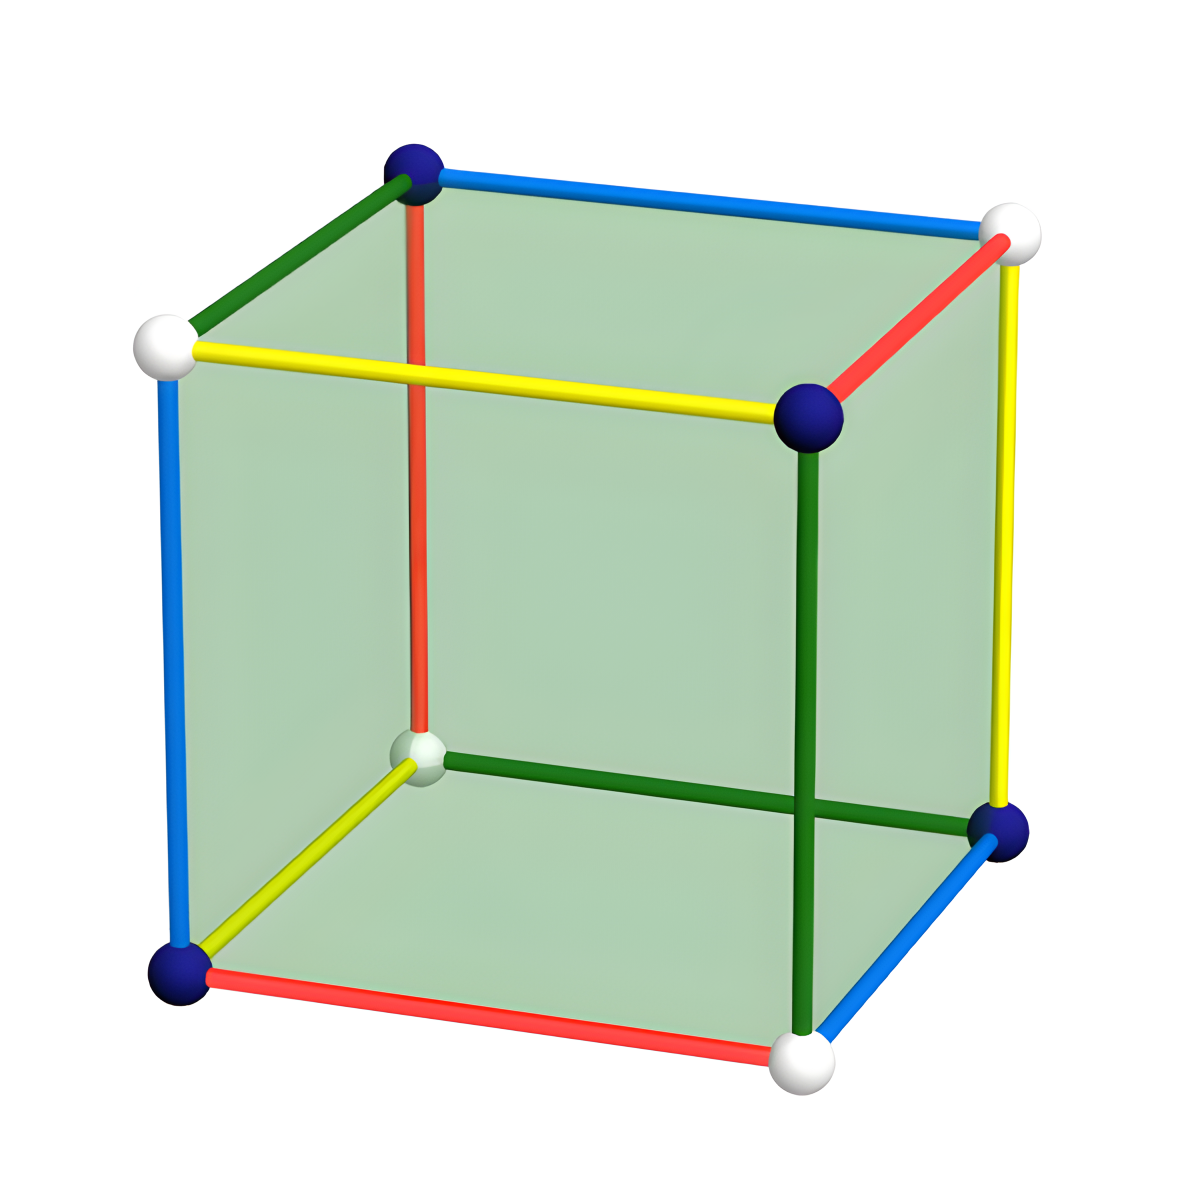
\includegraphics[height= 6.5cm]{cube-3-2.png}
        \caption{The hypercubic manifold $\mathbb{HM}^1$ (analysis-situs)}
        \label{fig:H1M}
    \end{center}
    \end{figure}
\end{frame}
\begin{frame}
    \frametitle{Intro (9) : Goal of the internship}
    \begin{exampleblock}{Goals}
        \begin{itemize}
            \item We know how to define Eilenberg Mac-Lane spaces for finite groups in HoTT but the construction is not well understood
            \pause
            \item We would like to achieve a "nicer" construction that would yield a handy induction principle
            \pause
            \item This would open up to define "Higher Group" actions and computer checked cohomology calculations.
            \pause
            \item It turns out that $\pi_1(\mathbb{HM}^1)=\mathcal{Q}$ and that by computing the "homotopy fiber" of a certain map my advisors have a way to provide such a "nice" construction in the case of the group $\mathcal Q$.
        \end{itemize}
    \end{exampleblock}
\end{frame}
\section{A brief overview of HoTT/cubical type theory}
    \subsection{Informal Type Theory}
        \subsubsection{Basics}
        \begin{frame}
            \frametitle{Some constructions on types}
            \begin{exampleblock}{Function types}
                Given types $A,B$ one has a type $A \rightarrow B$ of functions from $A$ to $B$.
            \end{exampleblock}
            \pause
            \begin{exampleblock}{Product types}
                Given types $A,B$ one has a product type $A \times B$. 
            \end{exampleblock}
            \pause
            \begin{exampleblock}{Dependant pair Types}
                If $B$ is a type family over a type $A$ (that is a function $B : A \rightarrow \mathcal{U}$) we have a type of dependant pairs $\sum_{x : A} B(x) $.
            \end{exampleblock}
            \pause
            \begin{exampleblock}{Coproduct types}
                Give types $A,B$ one has a coproduct type $A+B$ given by the constructors :
                \begin{itemize}
                    \item inl : $A \rightarrow A+B$
                    \item inr : $B \rightarrow A+B$
                  \end{itemize}
            \end{exampleblock}
        \end{frame}
        \begin{frame}
            \frametitle{Manipulating types}
            \begin{block}{Introduction rules}
                They encapsulate how to build an element of a certain type.
                \begin{itemize}
                    \item To build an element of $ f: A \rightarrow B$ one needs an expression $\phi(x)$ such that $a : A \vdash \phi(a) : B$ and to set $f :\equiv \lambda x. \phi(x)$
                    \item To build an element of $A \times B$ one needs elements $a : A$ and $b : B$ to form $(a,b) : A \times B$
                \end{itemize}
            \end{block}
            \pause
            \begin{block}{Induction principles}
                They encapsulate how to build \textbf{dependent} functions from a source type $A$.
                \begin{itemize}
                    \item To build a function of type $f : \prod_{x : A\times B} P(x)$ one only needs to give its value on pairs $(a,b)$. 
                \end{itemize}
            \end{block}
        \end{frame}

        \begin{frame}
            \frametitle{A working example : product types (1)}
            \begin{exampleblock}{Projections}
                We can define projections $\mathrm{pr}_1 : A\times B \rightarrow A$ and $\mathrm{pr}_2 : A\times B \rightarrow B$ by the \textbf{induction} principle for product types by setting $\mathrm{pr}_1((a,b)) :\equiv a$ and $\mathrm{pr}_2((a,b)) :\equiv b$.
            \end{exampleblock}
            % \pause
            % \begin{exampleblock}{Propositional uniqueness for product types}
            %    We have a type theoretic statement that expresses that the type $A \times B$ is the type of "pairs of elements of $A$ and $B$" : 
             %   $$ \mathrm{uniq}_{A\times B} : \prod_{x : A \times B} \big(x =_{A \times B} (\mathrm{pr}_1(x),\mathrm{pr}_2(x))\big) $$
            %\end{exampleblock}
        \end{frame}
        %\begin{frame}
            %\frametitle{A working example : product types (2)}
            %Sketch of proof : 
            %\begin{itemize}
                %\item By induction, we only need to build an element : 
                %$$\mathrm{uniq}_{A \times B} ((a,b)) : (a,b)=(\mathrm{pr}_1(a,b),\mathrm%{pr}_2(a,b))$$
                %\pause
                %\item By the definition of the projections, the goal type reduces to: 
                %$$(a,b)=_{A\times B} (a,b)$$
                %\pause
                %\item We now have an element $\mathrm{refl} : (a,b)=_{A\times B} (a,b)$ %\qed
         %   \end{itemize}
        
        %\end{frame}
    %\subsubsection{Propositions as types}
    %    \begin{frame}
    %        \frametitle{Propositions as types (1)}
    %        \begin{figure}[h]
    %            \begin{center}
    %                \begin{tabular}{|c|c|}
    %                    \hline Types & Logic  \\
    %                    \hline$A$ & $A$ is a proposition  \\
    %                    \hline$a: A$ & $a$ is a proof of $A$ \\
    %                    \hline $\textbf{0},\textbf{1}$ & $\perp, \top$ \\
    %                    \hline$A+B$ & $A \vee B$  \\
    %                    \hline$A \times B$ & $A \wedge B$  \\
    %                    \hline$A \rightarrow B$ & $A \Rightarrow B$ \\
    %                    \hline$A \rightarrow \textbf{0}$ & $\lnot A$ \\
    %                    \hline
    %                \end{tabular}
    %            \end{center}
    %        \end{figure}
    %    \end{frame}
    %    \begin{frame}
    %        \frametitle{Propositions as types (2)}
    %        \begin{center}
    %            \begin{tabular}{|c|c|}
    %                \hline Types & Logic  \\
    %                \hline$\prod_{x : A} P(x)$ & For all $x :A$, $P(x)$ holds  \\
    %                \hline$\sum_{x : A} P(x)$ & There exists $x : A$ such that $P(x)$ holds\\
    %                \hline
    %            \end{tabular}
    %        \end{center}
    %        \pause 
    %        \begin{exampleblock}{Observation}
    %            One can also think of the type $\sum_{x: a} P(x)$ as the type of all $x : A$ such that $P(x)$ holds.
    %        \end{exampleblock}
    %    \end{frame}
    %    \begin{frame}
    %        \frametitle{Propositions as types (3) : Semi-groups}
    %        \begin{definition}
    %            A \textbf{semigroup} is a type $A$ equipped with an associative binary operation $m : A\times A \rightarrow A$.
    %        \end{definition}
    %        \pause
    %        \begin{definition}[associativity]
    %            $$\mathrm{isAssoc}(m) : \prod_{x,y,z : A }m(x,m(y,z))=m(m(x,y),z)$$
    %        \end{definition}
    %        \pause
    %        \begin{definition}[Type of semigroups]
    %            $$\mathrm{SemiGroup} :\equiv \sum_{A : \mathcal{U}} \sum_{m : A \times A \rightarrow A} \mathrm{isAssoc}(m)$$
    %        \end{definition}
    %    \end{frame}
     \subsubsection{Identity types}
        \begin{frame}
            \frametitle{Identity types (1)} 
            \begin{exampleblock}{Definition}
                Given a type $A$ and elements $a, b : A$ there exists a type $a =_A b$ called the identity type of $a$ and $b$. We say that "$a$ is equal to $b$" if there exists some element $p : a =_A b$ 
            \end{exampleblock}
            \pause
            \begin{exampleblock}{Reflexivity}
                For any type $A$ and point $x : A$ there is an element $\mathrm{refl}_x : x=_A x$
            \end{exampleblock}
        \end{frame}
        \begin{frame}
            \frametitle{Identity types (2)}
            \begin{alertblock}{Path induction}
                To prove a predicate that depends on $x,y : A$ and $p : x=_A y$ one only needs to prove it in the case where $x \equiv y$ and $p \equiv \mathrm{refl}$.
            \end{alertblock}
            \pause
            \begin{example}[Functions preserve equals]
                For any $f :  A \rightarrow B$, $x,y :A$ and $p : a=_A b$ there is an element $$f(p) : f(a)=_B f(b)$$
            \end{example}
        \end{frame}
        \begin{frame}
            \frametitle{Identity types (3)}
            Sketch of proof : 
            \pause
            \begin{itemize}
                \item By path induction suppose that $x \equiv y$ and $p \equiv \mathrm{refl}$\\
                \pause
                \item We then have to provide an element of $f(x) =_B f(x)$\\
                \pause
                \item We conclude by setting $f(\mathrm{refl}_x) :\equiv \mathrm{refl}_{f(x)}$ 
                \\\qed
            \end{itemize}
        \end{frame}
    \subsection{HoTT/Cubical Type Theory}
    \subsubsection{The homotopical interpretation}
    \begin{frame}
        \frametitle{HoTT : The homotopical interpretation of Type Theory (1)}
        \begin{center}
            \begin{tabular}{|c|c|}
            \hline Types & Topology  \\
            \hline$A$ & a space $A$   \\
            \hline$a: A$ & $a$ is a point of $A$ \\
            \hline $p : x=_A y$ & $p$ is a path from $x$ to $y$ in the space $A$ \\
            \hline
            \end{tabular}
        \end{center}
        \pause
        \begin{figure}[h]
            \centering
            \begin{tikzpicture}[scale=0.7]
              \draw (0,0) ellipse (3.5cm and 2cm);
              \filldraw (-2.5,0) circle (1.5pt) node [below left] {$x$};
              \filldraw (2.5,0) circle (1.5pt) node [below right] {$y$};
              \filldraw [pattern={Lines[angle=60, distance=8pt]}] (-2.5,0) .. controls (-1,1.5) and (1,1.5) .. (2.5,0) .. controls (1,-1.5) and (-1,-1.5) .. (-2.5,0) -- cycle;
              \draw [thick, double] (0,1.152) -- (0,-1.152) node [at start, above] {$p$} node [midway, right] {$r$} node [at end, below] {$q$};
              \node (A) at (3.3,1.5) {$A$};
            \end{tikzpicture}
            \caption{two points $x,y : A$, two paths $p,q: x=_A y$ and a homotopy $r : p =_{x=_A y} q$}
        \end{figure}
    \end{frame}
    \begin{frame}
        \frametitle{HoTT : The homotopical interpretation of Type Theory (2)}
        \begin{center}
            \begin{tabular}{|c|c|}
              \hline Equality & Homotopy \\
              \hline reflexivity & constant path \\
              \hline symmetry  & path inversion \\
              \hline transitivity & concatenation of paths \\
              \hline
            \end{tabular}
        \end{center}
        \pause
        \begin{itemize}
            \item \textbf{Symmetry : } Given a path $p : x =_A y$, one has an inverse path $p^{-1} : y =_A x$ such that for any $x$, $\mathrm{refl}_x^{-1} \equiv \mathrm{refl}_x$.
            \item \textbf{Transitivity : } Given paths $p : x =_A y$ and $q : y =_A z$ one has a concatenated path $p \cdot q : x =_A z$ such that for any $x$, $\mathrm{refl}_x \cdot \mathrm{refl}_x \equiv \mathrm{refl}_x$.
        \end{itemize}
        \pause
        There are additional properties that one can prove such as $$p \cdot p^{-1} = \mathrm{refl}$$ that justify this whole interpretation.
    \end{frame}
    \subsubsection{Transport, Fibrations and Univalence}
    \begin{frame}
        \frametitle{Transports}
    \begin{exampleblock}{Equalities and dependent functions}
        Take $f : \prod_{x : A} P(x)$, $x,y : A$ and $p : x = y$. \\
        Note that we can't have a path between $f(x) : P(x)$ and $f(y) : P(y)$.
    \end{exampleblock}
    \pause
    \begin{alertblock}{Transport}
        By path induction, for any $x,y$ and $p : x=y$ one can define : 
        $$\mathrm{transport}^P : \prod_{a,b : A} \prod_{p : a=_A b} P(a) \rightarrow P(b)$$
        We may write $\mathrm{transport}^P(a,b,p)$ as $p_*$ if the context is clear.
    \end{alertblock}
    \pause
    \begin{example}
        The map $p_*$ encapsulates how are transported elements of the "fiber" $P(x)$ to the fiber $P(y)$ by going along the path $p : x=y$.
    \end{example}
    \end{frame}
    \begin{frame}
        \frametitle{Fibrations (1)}
        \begin{exampleblock}{Fibration}
            Take a continuous map $p : E \rightarrow B$. It is called a fibration if it has a certain path lifting property from the $\textbf{base space } B$ to the $\textbf{total space } E$. 
        \end{exampleblock}
        \pause
        \begin{alertblock}{Fibrations in HoTT}
            Take a type family $B$ over $A$ (that is $B : A \rightarrow \mathcal{U}$). \\ Then, the type $\sum_{x : A} B(x)$ equipped with its first projection $\mathrm{pr}_1$ is a fibration. \\
            \pause
            More precisely : \\
            Given $x : A$ and $u : P(x)$, for any $y : A$ and $p : x=y$, one has a path 
  $$\mathrm{lift}(p,u) : (x,u) = (y,p_*(u))$$
  such that $\mathrm{pr}_1(\mathrm{lift}(p,u)) = p$.
        \end{alertblock}
    \end{frame}
    \begin{frame}
        \frametitle{Fibrations (2)}
        \begin{center}
            \begin{tikzpicture}[scale=0.7]
              \draw (0,7) ellipse (4.4cm and 2.5cm);
              \draw (-1.7,7) ellipse (1.15cm and 1.05cm);
              \draw (1.7,7) ellipse (1.15cm and 1.05cm);
              \filldraw (-1.7,7) circle (1.5pt) node [above left] {$u$};
              \filldraw (1.7,7) circle (1.5pt) node [above right] {$p_*(u)$};
              \draw (-1.7,7) .. controls (-1,8) and (1,8) .. (1.7,7) node [midway, above] {$\mathrm{lift}(p,u)$};
            
              \draw [dash pattern=on 5pt off 3pt] (-1.7,0) -- (-1.7,7) (1.7,0) -- (1.7,7);
              \draw [very thick, ->] (-3,4.5) -- (-3,1.5) node [midway,left] {$\mathrm{pr}_1$};
            
              \draw (0,0) ellipse (4.4cm and 1.5cm);
              \filldraw (-1.7,0) circle (1.5pt) node [below left] {$x$};
              \filldraw (1.7,0) circle (1.5pt) node [below right] {$y$};
              \draw (-1.7,0) .. controls (-0.7,0.7) and (0.7,0.7) .. (1.7,0) node [midway, above] {$p$};
               
              \node (A) at (4.5,-1.5) {$A$};
              \node (B) at (5,5.5) {$\displaystyle\sum_{a:A} B(a)$};
              \node (C) at (-3.5,7) {$B(x)$};
              \node (D) at (3.5,7) {$B(y)$};
            \end{tikzpicture}
          \end{center}
    \end{frame}
    \begin{frame}
        \frametitle{Fibrations (3)}
        \begin{exampleblock}{Paths over paths}
            Now, given $f : \prod_{x : A} B(x)$ and $p : x = y$ there is a natural identification between points $f(x)$ and $p_*(f(x))$. \\
            \pause
            A path lying over $p$ should then factor through this path and consist of a path between $p_*(f(x))$ and a certain point $ u : P(y)$. \\
            \pause
            Dependent functions yield such paths : 
            $$\mathrm{apd}_f : \prod_{p : x=_A y} p_*(f(x))=f(y)$$
        \end{exampleblock}
    \end{frame}
    \begin{frame}
        \frametitle{Equivalences and Univalence}
        \begin{exampleblock}{Equivalences}
            We can build them from quasi-equivalences. Two types are quasi-equivalent if there exists maps $f : A \rightarrow B$ and $g : B \rightarrow A$ such that : 
            $$\prod_{x: A} g(f(x)) = x \quad \text{and} \quad \prod_{y : B} f(g(y))=y$$
        \end{exampleblock}
        \pause
        \begin{alertblock}{Univalence}
            One has : 
            $$\big ( A \simeq B \big ) \simeq \big ( A=B \big )$$
        \end{alertblock}
    \end{frame}
    \subsubsection{Higher Inductive Types}
    \begin{frame}
        \frametitle{Higher Inductive Types}
        \begin{exampleblock}{Idea}
            When dealing with HITs we allow ourselves to use paths constructors, paths between paths constructors and so on.
        \end{exampleblock}
        \pause
        \begin{alertblock}{The circle $\mathbb{S}^1$}
            The circle $\mathbb{S}^1$ is defined by the following HIT : \\
            \begin{minipage}{.45\linewidth}
                \begin{itemize}
                  \item $\mathrm{base} : \mathbb{S}^1$
                  \item $\mathrm{loop} : \mathrm{base} =_{\mathbb{S}^1} \mathrm{base}$
                \end{itemize}
              \end{minipage}
              \hfill
              \begin{minipage}{.45\linewidth}
                \begin{center}
                  \begin{tikzpicture}
                    \draw (0,0) ellipse (2.5cm and 0.5cm);
                    \filldraw (0,-0.5) circle (2pt) node [below right] {base};
                    \node (A) at (-2.5,0.7) [right] {loop};
                  \end{tikzpicture}
                \end{center}
            \end{minipage}
        \end{alertblock}
    \end{frame}
    \begin{frame}
        \frametitle{HITs : Induction Principle}
        \begin{alertblock}{We have a problem}
            When dealing with paths constructors and higher paths constructors, induction principles can become very hard to manipulate. 
        \end{alertblock}
        \pause
        \begin{exampleblock}{The case of $\mathbb{S}^1$}
            To define a map $f : \prod_{x : \mathbb{S}^1} P(x)$, one needs to specify its value $f(\mathrm{base}) : P(\mathrm{base})$. Then, what should you send $\mathrm{loop}$ to ? \\
            \pause
            Recall that by transport : 
            $$P(\mathrm{base}) \overset{\mathrm{loop}_*} \simeq P(\mathrm{base})$$
            Since $f$ is a dependent function, it should send $\mathrm{loop}$ to a dependent path between $\mathrm{loop}_*(f(\mathrm{base}))$ and $f(\mathrm{base})$.
        \end{exampleblock}
    \end{frame}
    \begin{frame}[fragile]
        \frametitle{Some other HITs (1)}
        \begin{alertblock}{Coequalizers}
            Given types $B,A$ and maps $f,g : B \rightarrow  A$ the (homotopy) \textbf{coequalizer} type $\mathrm{CoEq(f,g)}$ is given by the HIT:\\
            \begin{minipage}{.45\textwidth} 
                \begin{itemize}
                \item $c : A \rightarrow \mathrm{CoEq(f,g)}$
                \item $p : \prod_{b : B} c(f(b))=c(g(b))$
                \end{itemize}
            \end{minipage}
            \hfill 
            \begin{minipage}{.45\textwidth} 
                \begin{center}
                \begin{tikzcd}
                    B \arrow[r, "f"', shift right] \arrow[r, "g", shift left=2] & A \arrow[r, "c"] & {\mathrm{CoEq}(f,g)}
                \end{tikzcd}
                \end{center}
            \end{minipage}
        \end{alertblock}
        \pause
        \begin{exampleblock}{The circle as a coequalizer}
            \begin{center}
                \begin{tikzcd}
                    \textbf{1} \arrow[r, "1"', shift right] \arrow[r, "1", shift left=2] & \textbf{1} \arrow[r, "c"] & {\mathrm{CoEq}(1,1) \simeq \mathbb{S}^1}
                \end{tikzcd}
            \end{center}
        \end{exampleblock}
    \end{frame}
    \begin{frame}[fragile]
        \frametitle{Cubical Type Theory : Completing Squares}
        \begin{alertblock}{Filling property}
            Given an incomplete square of paths 
            \begin{center}
                \begin{tikzcd}
                  a \arrow[r, "p"] \arrow[d, "q"'] & b \arrow[d, "r"] \\
                  c                                & d               
                  \end{tikzcd}  
            \end{center}
            Then there is a unique path $s$ from $c$ to $d$ that completes the square by making it commute, that is :
            $$ q \cdot s = p \cdot r $$
        \end{alertblock}
    \end{frame}
    \begin{frame}[fragile]
        \frametitle{Why do we complete squares?}
        \begin{center}
            \begin{tikzcd}
              {a_{0,1}} \arrow[rr, "s"]                                            & {}                                            & {a_{1,1}}                                            \\
                                                                                   &                                               &                                                      \\
              {a_{0,0}} \arrow[rr, "r"'] \arrow[uu, "p \equiv c \hspace{3pt} i_0"] & {} \arrow[uu, "c \hspace{3pt} i", shift left] & {a_{1,0}} \arrow[uu, "q \equiv c \hspace{3pt} i_1"'] \\
              i_0 \arrow[rr, bend right]                                           & i                                             & i_1                                                 
              \end{tikzcd} 
          \end{center}
    \end{frame}
    \begin{frame}[fragile]
        \frametitle{Some other HITs (2) : The torus $\mathbb{T}^2$}
        \begin{figure}[h]
            \begin{center}
              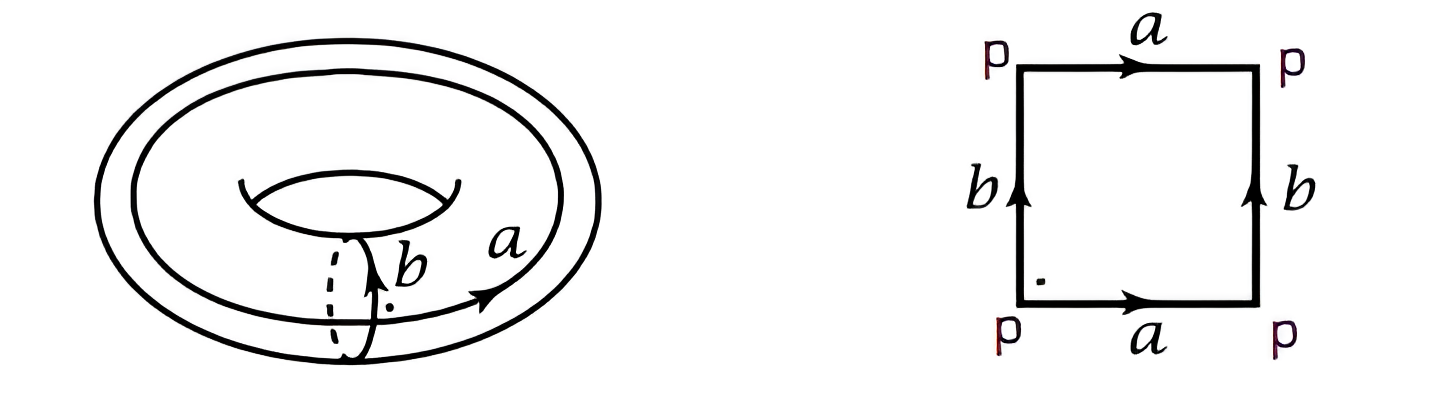
\includegraphics[height= 2.5cm]{torus.png}
              \caption{The torus $\mathbb{T}^2$ and its presentation as a cell complex (Hatcher)}
            \end{center}
          \end{figure}
        \pause
        This leads to the following HIT definition of $\mathbb{T}^2$ :
        \begin{itemize}
            \item $ p : \mathbb{T}^2$
            \item $a : p = p$
            \item $b : p = p $
            \item $\mathrm{fill} :  a \cdot b = b \cdot a$
        \end{itemize}
    \end{frame}
    \begin{frame}[fragile]
        \frametitle{Some other HITs (3) : The Torus $\mathbb{T}^2$}
        In cubical type theory (and cubical) agda, we fill squares !
        \pause
        This gives another definition of the Torus with an already built-in "filled square Type".\\
        \begin{lstlisting}[mathescape=true]
            data Torus2 : Type where
            p : Torus2
            a : $ p \equiv p$
            b : $p \equiv p$
            fill : Square b b a a
        \end{lstlisting}
    \end{frame}
    \begin{frame}
        \frametitle{Somer other HITs : Fundamental groups}
        \begin{exampleblock}{Fundamental group presentation}
            Take a HIT with one point constructor. Then its fundamental group has a presentation given by its paths constructors and the relations between paths.
        \end{exampleblock}
        \pause
        $$\pi_1(\mathbb{S}^1) = \mathbb{Z}$$
        \pause
        $$\pi_1(\mathbb{T}^2) = \mathbb{Z}^2$$
        \pause
        Given a presentation of $G$ we can build a space $H$ with $\pi_1(H) = G$.
    \end{frame}
    \section{Some work done during the internship}
    \subsection{Defining $\mathbb{HM}^1$}
    \begin{frame}
        \frametitle{The Hypercubic Manifold $\mathbb{HM}^1$}
        \begin{figure}[h]
        \begin{center}
            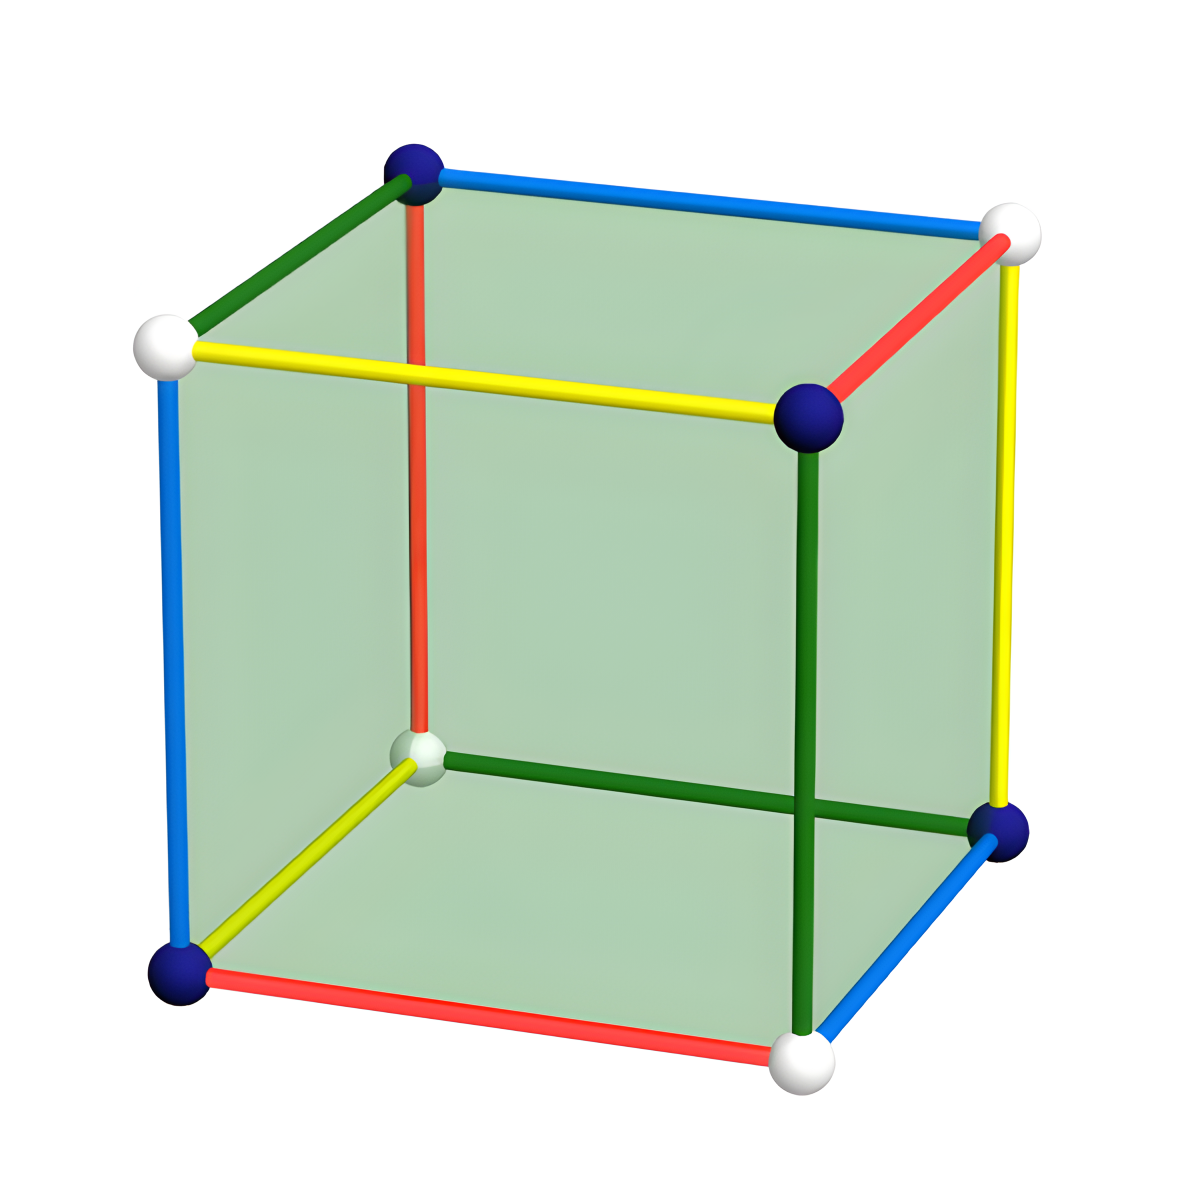
\includegraphics[height= 6.5cm]{cube-3-2.png}
            \caption{The hypercubic manifold $\mathbb{HM}^1$ (analysis-situs)}
            \label{fig:H1M}
        \end{center}
        \end{figure}
    \end{frame}
    \begin{frame}[fragile]
        \frametitle{Defining $\mathbb{HM}^1$ (1)}
        \begin{exampleblock}{The HIT/CW-complex correspondence}
            A first step is to notice that defining HITs and CW-complex is pretty much the same (as seen for the Torus).
        \end{exampleblock}
        \pause
        To begin with, we will name the vertex constructors $b^V$ and $w^V$ (for blue and white vertex) and the edge constructors $b^E$, $r^E$, $g^E$, $y^E$. 
        \pause
        \begin{exampleblock}{Challenges}
            \begin{itemize}
                \item Identifying opposite sides under a quater of a turn rotation
                \item Filling the cube
            \end{itemize}
        \end{exampleblock}
    \end{frame}
    \begin{frame}
        \frametitle{The Hypercubic Manifold $\mathbb{HM}^1$}
        \begin{figure}[h]
        \begin{center}
            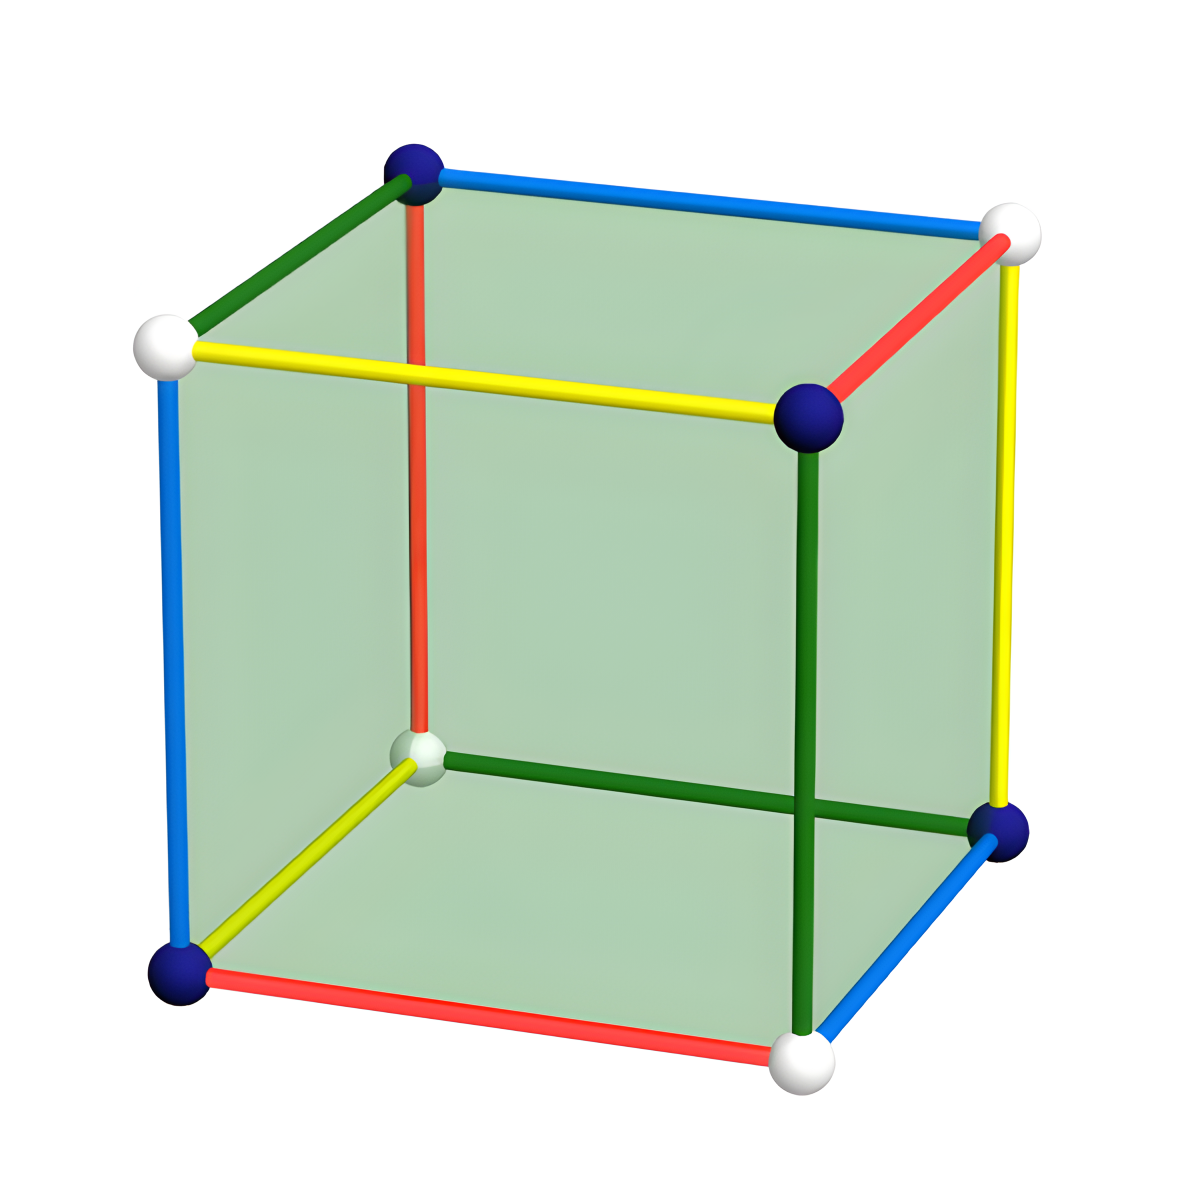
\includegraphics[height= 6.5cm]{cube-3-2.png}
            \caption{The hypercubic manifold $\mathbb{HM}^1$ (analysis-situs)}
            \label{fig:H1M}
        \end{center}
        \end{figure}
    \end{frame}
    \begin{frame}[fragile]
        \frametitle{Defining $\mathbb{HM}^1$ (2) : Rotation}
        Begin with a filled square, that is a commutative diagram of paths : 
        \begin{center}
            \begin{tikzcd}
              {} \arrow[r, "s"]                 & {}                 \\
              {} \arrow[u, "p"] \arrow[r, "r"'] & {} \arrow[u, "q"']
            \end{tikzcd}
          \end{center}
        \pause
        This in tantamount to having : $p \cdot s = r \cdot q$ \\
        \pause
        Let's rewrite it : $r^{-1} \cdot p = q \cdot s^{-1}$ \\
        \pause
        Yielding us the following filled square :
        \begin{center}
            \begin{tikzcd}
              {} \arrow[r, "p"]                      & {}                      \\
              {} \arrow[u, "r^{-1}"] \arrow[r, "q"'] & {} \arrow[u, "s^{-1}"']
              \end{tikzcd}
        \end{center} 
        \pause 
        We have just defined a map : 
        $$\boxed{\text{rot : Square $p$ $q$ $r$ $s$ $\rightarrow$ Square $\overline{r}$ $\overline{s}$ $q$ $p$}}$$
    \end{frame}
    \begin{frame}
        \frametitle{Defining $\mathbb{HM}^1$ (3) : Result}
        \begin{figure}[h]
            \begin{center}
              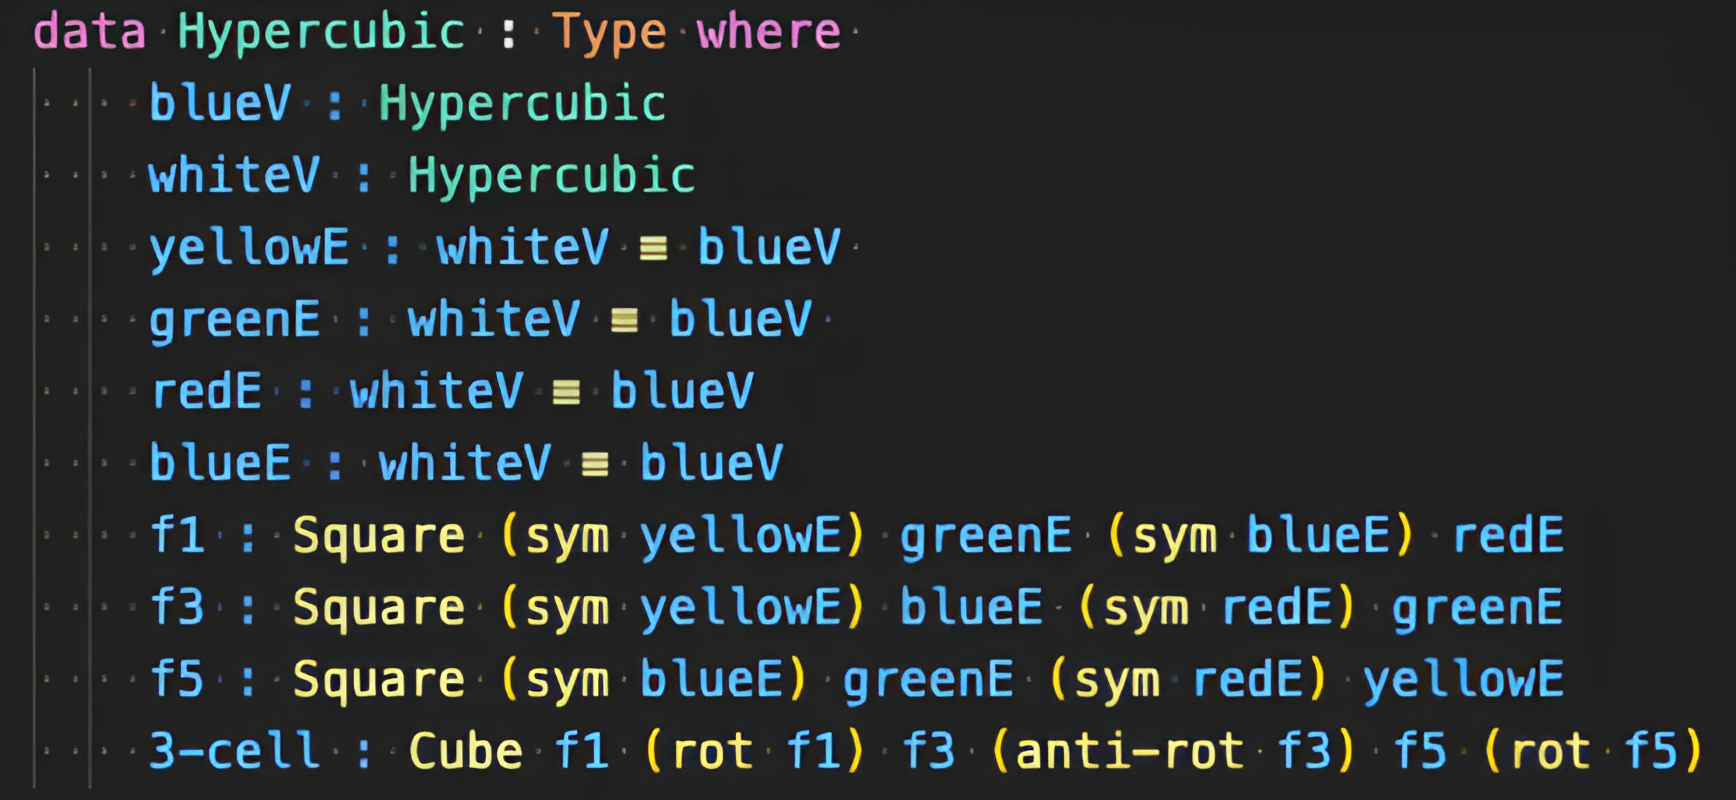
\includegraphics[height= 4.5cm]{images/Agda - VH.png}
              \caption{Synthetic description of the hypercubic manifold as a cubical HIT in cubical agda}
            \end{center}
          \end{figure}
    \end{frame}
    \subsection{A fiber calculation}
    \begin{frame}
        \frametitle{Homotopy fibers}
        \begin{exampleblock}{Homotopy fiber}
            Given a map $f : A \rightarrow B$ and $b : B$ the fiber of $f$ over $b$ is given by : 
            $$\mathrm{fib}_f(b) \hspace{3pt} :\equiv \sum_{x: A} f(x)=_B b$$
        \end{exampleblock}
        \pause
        The final goal of the internship was to compute such a fiber, it has not yet been computed but we will look at an instructive example instead.
    \end{frame}
    \begin{frame}
        \frametitle{A fiber calculation (1)}
        For a group $G$, $\mathrm{B}G$ denotes the Eilenberg Mac-lane space of $G$. \\
        \pause
        A famous result in homotopy theory is that : 
        $$\mathrm{B}\mathbb{Z} = \mathbb{S}^1$$
        \pause
        Let now $m$ be a nonnegative integer and $r \in \mathbb{Z}_m^{\times}$ (the integers mod $m$). Then we have a short exact sequence of groups : 
        $$\mathbb{Z} \xrightarrow{\times m} \mathbb{Z} \xrightarrow{1 \mapsto \overline r} \mathbb Z_m$$
        \pause
        Which, for  topological reasons, yields a fibration of Eilenberg Mac-Lane spaces:
        $$\mathbb{S}^1 \xrightarrow{\mathrm{base} \mapsto \mathrm{base}, \quad  \mathrm{loop} \mapsto \mathrm{loop}^m} \mathbb{S}^1 \xrightarrow{g} \mathrm{B}\mathbb{Z}_m$$
        This is in fact a fibration whose base space is $\mathrm{B}\mathbb{Z}_m$, of total space $\mathbb{S}^1$, and for which the fiber of $g$ over the canonical element $*$ of $\mathrm{B}\mathbb{Z}_m$ should be $\mathbb{S}^1$. 
    \end{frame}
    \begin{frame}
        \frametitle{A fiber calculation (2)}
        By definition, the fundamental group at $*$ in $\mathrm{B}\mathbb{Z}_m$ is $\mathbb{Z}_m$, we choose a presentation of it as the powers of $s_m$ the succesor mod $m$. Then the map $g$ is given by : 
        $$g(\mathrm{base}) :\equiv *, \quad \mathrm{ap}_g(\mathrm{loop}) :\equiv \mathrm{ua}(s_m^r)$$
        \pause
        We can now begin ! 
    \end{frame}
    \begin{frame}[fragile]
        \frametitle{A fiber calculation (3) : diagrams}
        If $P : \mathrm{B}\mathbb{Z}_m \rightarrow \mathcal{U}$ is defined by $P :\equiv x \mapsto  x = s_m$ then we have a fibration over $\mathbb{S}^1$ given by $P \circ g$ whose total space is by definition:
        $$\sum_{x : \mathbb{S}^1} P \circ g (x) :\equiv \sum_{x : \mathbb{S}^1}(g(x)=s_m) :\equiv \mathrm{fib}_g(s_m)$$
        \pause 
        Recalling that $\mathbb{S}^1$ is obtained as a coequalizer type, we obtain the following commutative diagram : 
        \begin{center}
            \begin{tikzcd}
              1 \arrow[r, shift left] \arrow[r, shift right] & 1 \arrow[r, "\mathrm{base}"] \arrow[rd, "s_m =s_m"'] & \mathbb{S}^1 \arrow[r, "g"] \arrow[d, "P \circ g" description] & \mathrm{B} \mathbb{Z}_m \arrow[ld, "P"'] \\
                                                             &                                                      & \mathcal U                                                     &                                         
            \end{tikzcd}
          \end{center}
    \end{frame}
    \begin{frame}[fragile]
        \frametitle{A fiber calculation (4) : The flattening lemma}
        \begin{alertblock}{Flattening Lemma}
            Suppose given a fibration over a coequalizer type: 
            \begin{center}
              \begin{tikzcd}
                B \arrow[r, "f", shift left] \arrow[r, "g"', shift right] & A \arrow[r, "c"] & W \arrow[r, "P"] & \mathcal U
              \end{tikzcd}
            \end{center}
            Then, one has a coequalizer diagram between the total spaces: 
            \begin{center}
              \begin{tikzcd}
                \displaystyle \sum_{b : B} P \circ c \circ f (a) \arrow[rrr, "{(b,x) \mapsto(g(b),p_b^*(x))}", shift left=3] \arrow[rrr, "{(b,x) \mapsto (f(b),x)}"', shift right=3] &  &  & \displaystyle \sum_{a : A} P \circ c (a) \arrow[rr] &  & \displaystyle \sum_{w : W} P(w)
              \end{tikzcd}
            \end{center}
          \end{alertblock}
    \end{frame}
    \begin{frame}[fragile]
        \frametitle{A fiber calculation (5)}
        In our case, the lemma yields the following coequalizer diagram :
        \begin{center}
        \begin{tikzcd}
        s_m=s_m \arrow[rr, "\mathrm{Id}", shift left] \arrow[rr, "p \mapsto p^r"', shift right] &  & s_m=s_m \arrow[r] & \mathrm{fib}_g(s_m)
        \end{tikzcd}
        \end{center}
        \pause
        Given that :
        $$(s_m = s_m) \simeq (s_m \simeq s_m) \simeq \langle s_m \rangle \simeq \mathbb{Z}_m$$
        \pause
        We get that $\mathrm{fib}_g(s_m)$ is equivalent to the HIT $W$ defined by the following constructors : 
        \begin{itemize}
        \item $c : \mathrm{Fin} \hspace{2pt} m \mapsto W$
        \item $ p : \prod_{x : \mathrm{Fin}\hspace{2pt} m} (c(x) = c(s_m^r(x)))$
        \end{itemize}
    \end{frame}
    \begin{frame}[fragile]
        \frametitle{A fiber calculation (6)}
        Since $r$ is coprime to $m$, it turns out that $s_m^r$ is of order $m$ so the orbit of $c(0)$ under the action of the group $\langle s_m^r \rangle$ is the whole type $W$.
        \pause
        \begin{center}
            \begin{tikzpicture}[scale=0.55]
              \draw (-2,0.5) .. controls (-2,1) and (-1,2) .. (-0.5,2) node [midway, above left] {$p_0$};
              \draw (0.5,2) .. controls (1,2) and (2,1) .. (2,0.5) node [midway, above right] {$p_1$};
              \draw (2,-0.5) .. controls (2,-1) and (1,-2) .. (0.5,-2) node [midway, below right] {$p_2$};
              \draw (-0.5,-2) .. controls (-1,-2) and (-2,-1) .. (-2,-0.5) node [midway, below left] {$p_3$};
              \node (A) at (-2,0) {$c(0)$};
              \node (A) at (0,2) {$c(1)$};
              \node (A) at (2,0) {$c(2)$};
              \node (A) at (0,-2) {$c(3)$};
            \end{tikzpicture}
          \end{center}
          \pause
          Hence : 
          $$\boxed{\mathrm{fib}_g(s_m) \simeq \mathbb{S}^1}$$
    \end{frame}
    \begin{frame}
        \frametitle{A fiber calculation (7) : sketch of proof}
        The idea is that the general case should come from the case $r=1$.\\
        \pause
        For $r=1$, we have that :
        $$p_0 \cdot p_1 \cdot \ldots \cdot p_m : c(0)=c(0)$$ 
        and we can successively contract each path  : 
        $$p_i : c(i)\rightarrow c(\overline{i+1}_r)$$
        to end up with a type with a constructor $c(0)$ and a path $p_0 : c(0) = c(0)$, which is the circle.
    \end{frame}
    \begin{frame}
        \frametitle{A fiber calculation (8) : An extension}
        Let's consider the case where $r$ and $m$ are not coprime. \\
        In that case, let $\delta$ be the $\gcd$ of $r$ and $m$, then $s_m^r$ is now only of order $\frac m{\delta}$. \\
        \pause
        Hence, our type is now composed of $\delta$ disjoint orbits of size $\frac m{\delta}$, each orbit looking like the types we were previously looking at. \\
        \pause
        We then naturally obtain : 
        $$\boxed{\mathrm{fib}_g(s_m) = \bigplus_{i=1}^{\delta} \mathbb{S}^1}$$
    \end{frame}
    \section{Conclusion}
    \begin{frame}[fragile]
        \frametitle{Towards $\mathbb{HM}^1$ as $\faktor{\mathbb{S}^3}{\mathcal{Q} \acts \mathbb{S}^3}$}
        The final bit of the work would consist in an other fiber calculation that expresses $\mathbb{HM}^1$ as a homotopy quotient of $\mathbb{S}^3$ under an action of $\mathcal{Q}$. 
        \pause
        \begin{center}    
        \begin{tikzcd}
                \mathbb{HM}^1 \arrow[rr, "f"] &  & \mathrm{B}\mathcal{Q}
            \end{tikzcd}
        \end{center}
        \pause
        $$\mathcal{Q} \acts \mathrm{fib}_f(*) :\equiv \sum_{x : \mathbb{HM}^1} f(x) = *$$
        \pause
        $$ \mathbb{HM}^1 \simeq \faktor{\mathrm{fib}_f(*)}{\mathcal{Q} \acts \mathrm{fib}_f(*)}$$
    \end{frame}
\end{document}